\chapter{對稱性破缺、戈德斯通玻色子與規範不變性}

我們想了解類光子的粒子如何獲得質量。這是我們要探討的問題，但不是合理的起點。直接加入規範場質量項，似乎會破壞使理論自洽的規範不變性。要看出如何化解這個問題，我們得先掌握兩個概念：
\begin{enumerate}
  \item 自發對稱性破缺，尤其是連續對稱性的自發破缺；
  \item 規範不變性：對稱操作可以隨時空位置而改變。
\end{enumerate}
這兩個概念都不能只用一句口號帶過。我們會從磁體出發，建立第一個概念，再將它轉化為標量場論，並找出無質量的戈德斯通模式。接著，我們會將相同的 \(U(1)\) 對稱性推廣為局域對稱性，這會迫使我們引入向量勢和協變導數。最後才會把這兩條脈絡放在一起。它們真正的結合---希格斯現象---將在下一講討論。

\section{定律具有對稱性，基態卻不對稱}

\subsection{雙態磁體}

先從小磁體組成的點陣談起。每個自旋都可以朝上或朝下，相鄰自旋朝向相同時，能量較低。在三維立方點陣中，每個自旋有六個最近鄰，但確切的配位數並不重要。重要的是這條規則：
\begin{equation}
  E_{\parallel}<E_{\rm antiparallel}.
\end{equation}
若將每個自旋反轉，微觀規則仍然不變：
\begin{equation}
  \uparrow\longleftrightarrow\downarrow.
\end{equation}
然而，最低能量的構型各自都不具對稱性，分別是
\begin{equation}
  \{\uparrow\uparrow\uparrow\cdots\},
  \qquad
  \{\downarrow\downarrow\downarrow\cdots\}.
\end{equation}
方程容許這兩種構型，但低溫下的宏觀樣品必須擇一。

這種選擇極其敏感。把遠處的一個自旋固定為朝上，它的鄰居就傾向跟著朝上；鄰居的鄰居也傾向跟著它們，這個影響便在樣品中傳開。相較於整個系統，任意微小的微擾都可能決定整個基態的取向。這就是\emph{自發}對稱性破缺所指的不穩定性。

\begin{classroomqa}
\audiencequestion{中性粒子能在磁場中定向嗎？
\lecturetimestamp{00:05:14}}
\lecturerresponse{能。電中性不代表沒有磁矩。中子雖然電中性，卻因內部帶電的組成粒子而具有磁矩。因此，磁場可以區分它的不同自旋取向。}
\end{classroomqa}

\begin{classroomqa}
\audiencequestion{如果系統改變取向，這種變化會同時發生在各處嗎？可以有好幾個重新取向的波同時存在嗎？
\lecturetimestamp{00:05:41--00:06:38}}
\lecturerresponse{變化會逐步傳播。一個區域會帶動鄰近區域，就像三維的多米諾骨牌陣列，擾動會以波的形式傳開。不同區域可能各自開始選擇取向，因此在某一種取向勝出之前，可能同時存在好幾個波前和疇。等對稱性變成連續對稱性時，我們還會回頭談這些波。}
\end{classroomqa}

\subsection{顯式對稱性破缺是另一種理論}

現在把樣品放在一個朝上的外加磁場中。對單獨一個自旋而言，朝上時的能量本來就較低。變換 \(\uparrow\leftrightarrow\downarrow\) 不再使能量保持不變：偏好已經寫進定律本身。這就是\emph{顯式}對稱性破缺。

即使不知道樣品是如何製備的，也能檢驗兩者的差異。取一個很大的樣品，將左邊界固定為朝上，右邊界固定為朝下。如果體內的磁場明確偏好朝上，右側的邊界條件只能影響很短的距離。宏觀的朝下區域會付出與其體積成正比的能量，因此體相不可能維持分成兩個能量同樣有利的相。

沒有外加偏置時，朝上和朝下的體相能量相同。此時受邊界條件約束的最低能量狀態，會包含一個朝上疇、一個朝下疇，以及兩者之間有限寬度的過渡層。界面不一定位於幾何中心，但沒有體積壓力迫使其中一相消滅另一相。這個界面稱為\emph{疇壁}，是這種離散對稱性破缺的典型缺陷。

\begin{figure}[htbp]
\centering
\begin{adjustbox}{max width=\linewidth}
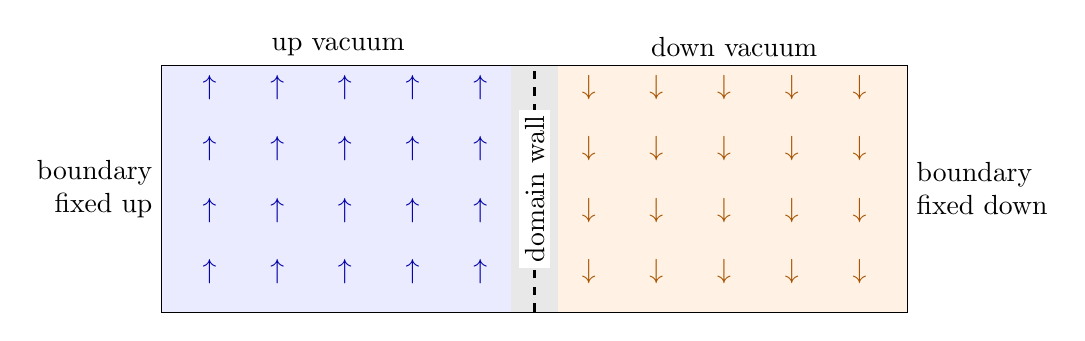
\begin{tikzpicture}[x=0.86cm,y=0.78cm]
  \draw[thick] (0,0) rectangle (11,4);
  \fill[blue!8] (0,0) rectangle (5.15,4);
  \fill[orange!10] (5.85,0) rectangle (11,4);
  \fill[gray!18] (5.15,0) rectangle (5.85,4);
  \foreach \x in {0.7,1.7,2.7,3.7,4.7}
    \foreach \y in {0.65,1.65,2.65,3.65}
      \node[blue!65!black] at (\x,\y) {$\uparrow$};
  \foreach \x in {6.3,7.3,8.3,9.3,10.3}
    \foreach \y in {0.65,1.65,2.65,3.65}
      \node[orange!65!black] at (\x,\y) {$\downarrow$};
  \draw[dashed,thick] (5.5,0) -- (5.5,4);
  \node[above] at (2.6,4) {up vacuum};
  \node[above] at (8.45,4) {down vacuum};
  \node[rotate=90,fill=white,inner sep=2pt] at (5.5,2) {domain wall};
  \node[left,align=right] at (0,2) {boundary\\fixed up};
  \node[right,align=left] at (11,2) {boundary\\fixed down};
\end{tikzpicture}
\end{adjustbox}
\caption{離散對稱性自發破缺的邊界檢驗。兩種體相取向的能量相同，因此疇壁可以分隔宏觀疇。}
\end{figure}

\begin{classroomqa}
\audiencequestion{這個論證是否只適用於最近鄰之間的相互作用？\lecturetimestamp{00:18:18}}
\lecturerresponse{不。若次近鄰相互作用也偏好排列方向一致，細節會有所改變，但結論不變。若不同作用距離之間彼此競爭，情況就更有意思了---例如，最近鄰偏好排列方向一致，次近鄰卻偏好反向排列。這會造成阻挫和更複雜的有序相，但不影響我們在此所區分的基本概念。}
\end{classroomqa}

\begin{classroomqa}
\audiencequestion{\emph{自發}是指疇壁內部的大導數嗎？\lecturetimestamp{00:19:05}}
\lecturerresponse{不是。這指的是底層能量對上--下並無偏好，但所選定的基態卻有。對任意小的擾動都會產生劇烈響應，這揭示了一種不穩定性。梯度只是告訴我們介面的代價有多大。}
\end{classroomqa}

\begin{classroomqa}
\audiencequestion{材料原本就處於兩種狀態之一嗎？還是它一開始的狀態並不確定？\lecturetimestamp{00:19:40}}
\lecturerresponse{這取決於它經歷過什麼。在高溫下，熱運動可能使朝上和朝下的自旋混雜，平均磁化強度幾乎為零。材料冷卻時，不同區域會選擇不同取向，形成疇壁，疇也會逐漸變大。偶然因素和微小的環境微擾，會決定最後哪個真空佔據樣品的大部分。}
\end{classroomqa}

\section{用標量場論重述相同的論證}

以實標量場 \(\phi(\bm{x},t)\) 取代自旋。固定度規與歸一化慣例後，寫成
\begin{equation}
\begin{aligned}
  \mathcal L
  &=\frac12\,\partial_\mu\phi\,\partial^\mu\phi-V(\phi),
  \\
  \mathcal E
  &=\frac12\dot\phi^{\,2}+\frac12(\nabla\phi)^2+V(\phi).
\end{aligned}
  \label{eq:l07-real-scalar}
\end{equation}
\(\mathcal L\)中的相對論簡寫包含正號的時間導數項和負號的空間梯度項；哈密頓量的能量密度中，兩項的貢獻則都是正的。

選擇一個具有兩個簡併極小值的偶勢：
\begin{equation}
  V(\phi)=\frac{\lambda}{4}\left(\phi^2-f^2\right)^2,
  \qquad \lambda>0.
  \label{eq:l07-double-well}
\end{equation}
拉格朗日量在 \(\phi\mapsto-\phi\) 之下保持不變，而任何一個均勻真空
\begin{equation}
  \phi(\bm{x})=+f,
  \qquad\hbox{or}\qquad
  \phi(\bm{x})=-f
\end{equation}
都會選擇其中一側。相較之下，若勢在 \(\phi=0\) 處只有一個極小值，真空便具有對稱性，也就沒有自發對稱性破缺。

把樣品一側的場固定為 \(\phi=+f\)，另一側固定為 \(\phi=-f\)。場無法毫無代價地跳變，因為
\begin{equation}
  E_{\rm wall}
  =\int dx\left[
      \frac12\left(\frac{d\phi}{dx}\right)^2+V(\phi)-V(f)
    \right].
  \label{eq:l07-wall-energy}
\end{equation}
若發生突跳，\(d\phi/dx\) 就會非常大。因此，最低能量的疇壁會將變化分散在有限寬度內，在梯度能和跨越兩個極小值之間的勢能代價間取得平衡。式~\eqref{eq:l07-double-well}所示勢能的熟知扭結解為
\begin{equation}
  \phi_{\rm wall}(x)
  =f\tanh\!\left[f\sqrt{\frac{\lambda}{2}}\,(x-x_0)\right],
  \label{eq:l07-kink}
\end{equation}
這具體呈現了黑板上所描述的平滑過渡。
\editorialnote{講課時是根據勢能的形狀和梯度項來論證，並未求解場方程。此處列出方程\eqref{eq:l07-kink}作為該模型的標準解，讓定性的疇壁有具體形式，同時不改變原本的論證。}

稍微傾斜雙勢阱，其中一個極小值就會較低。此時拉格朗日量本身已不具對稱性。疇壁仍可能暫時存在，但能量較高的假真空會對它施加壓力，使疇壁移動，偏好的相也隨之擴大。這就是場論中由外加磁場造成顯式對稱性破缺的情形。

到目前為止，我們討論的都是離散對稱性。粒子物理學主要涉及連續群，例如 \(U(1)\)、\(SU(2)\) 和 \(SU(3)\)。連續對稱性會改變缺陷的型態，並帶來一種新的粒子。

\section{複數場與全域 \texorpdfstring{\(U(1)\)}{U(1)}}

\subsection{內部平面中的旋轉}

令
\begin{equation}
  \phi=\phi_R+i\phi_I,
  \qquad
  \phi^*=\phi_R-i\phi_I,
  \qquad
  \phi^*\phi=\phi_R^2+\phi_I^2.
  \label{eq:l07-components}
\end{equation}
\(\phi_R\) 軸和 \(\phi_I\) 軸構成內部場空間，而不是普通空間中的兩個方向。複數標量場只是將兩個實標量場合併表示，讓內部平面中的旋轉清楚呈現。

\begin{figure}[htbp]
\centering
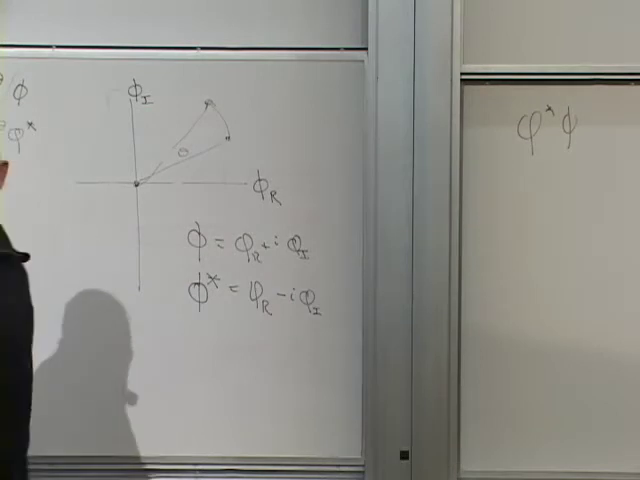
\includegraphics[width=0.80\textwidth]{lecture_07_figure_02.png}
\caption{內部 \((\phi_R,\phi_I)\) 平面上的複數場。黑板上列出 \(\phi\) 和 \(\phi^*\) 的分解，以及不變半徑 \(\phi^*\phi\)。}
\lectureframe{00:33:33}
\end{figure}

採用以下拉格朗日量：
\begin{equation}
  \mathcal L
  =\partial_\mu\phi^*\,\partial^\mu\phi
   -V(\phi^*\phi).
  \label{eq:l07-complex-lagrangian}
\end{equation}
對複數場而言，不需要通常會出現的因子 \(1/2\)，因為這一個乘積已經包含兩個實分量的動能項。變換
\begin{equation}
  \phi'(x)=e^{i\theta}\phi(x),
  \qquad
  \phi^{*\prime}(x)=e^{-i\theta}\phi^*(x)
  \label{eq:l07-global-u1}
\end{equation}
會將每個場值都旋轉相同的角度。此處的 \(\theta\) 在空間和時間中都是常數。撇號表示變換後的場，不是導數。

由於 \(\theta\) 是常數，
\begin{equation}
  \partial_\mu\phi'=e^{i\theta}\partial_\mu\phi,
  \qquad
  \partial_\mu\phi^{*\prime}
  =e^{-i\theta}\partial_\mu\phi^*.
\end{equation}
動能項中的相位會相消，而且
\(\phi^{*\prime}\phi'=\phi^*\phi\)。因此，任何只依賴 \(\phi^*\phi\) 的勢都具有相同的對稱性。若有項只依賴 \(\phi_R\)，就會在內部平面中選定一個方向，造成顯式對稱性破缺。

\subsection{單一極小值與一圈極小值}

對稱勢在性質上有兩種截然不同的情況。第一種的唯一極小值在原點，例如
\begin{equation}
  V_{\rm unbroken}=m^2\phi^*\phi,
  \qquad m^2>0.
\end{equation}
它的圖形是旋轉對稱的拋物面。真空 \(\phi=0\) 在任意旋轉下都保持不變，因此對稱性沒有破缺。

現在改選
\begin{equation}
  V_{\rm broken}
  =-a\,\phi^*\phi+b(\phi^*\phi)^2,
  \qquad a,b>0.
  \label{eq:l07-mexican-hat}
\end{equation}
負的二次項會使場離開原點，正的四次項則阻止場趨向無窮大。令 \(r^2=\phi^*\phi\)，極小化後得到
\begin{equation}
  \frac{dV}{d(r^2)}=-a+2br^2=0,
  \qquad
  r^2=f^2=\frac{a}{2b}.
  \label{eq:l07-vacuum-radius}
\end{equation}
因此，極小值構成一個圓。勢能完全具有旋轉對稱性，但均勻基態仍必須在圓上選定一點。

\begin{figure}[htbp]
\centering
\includegraphics[width=0.72\textwidth]{lecture_07_figure_06.png}
\caption{將對稱性破缺的勢能畫成旋轉曲面。原點不穩定，簡併極小值則構成環形谷底。}
\lectureframe{00:37:25}
\end{figure}

可以把場想成普通空間每一點上的一支小箭頭，箭頭位於這個內部平面中。勢能要求每支箭頭的長度都是 \(f\)。梯度能則要求相鄰箭頭的方向幾乎相同。因此，基態在各處都有相同的角度，但定律並未偏好任何特定角度。這就是連續對稱性的自發破缺。

\section{從疇壁到平滑扭轉}

再做一次邊界實驗。在左邊界把場固定於一個真空點 \(A\)，在右邊界則固定於另一個真空點 \(B\)。若場局部跳變，梯度就會很大。然而，不同於離散對稱性的情形，場可以沿著圓連續變化，同時始終留在勢能的谷底。

在低能情況下，將場寫成 \(\phi=f e^{i\alpha(x)}\)。在一維空間中，相關的能量為
\begin{equation}
  E[\alpha]
  =f^2\int_0^L dx\,\left(\frac{d\alpha}{dx}\right)^2.
  \label{eq:l07-angle-functional}
\end{equation}
固定兩端的角度後，變分可得
\begin{equation}
  \frac{d^2\alpha}{dx^2}=0,
  \qquad
  \alpha(x)=\alpha_A+
    \frac{\alpha_B-\alpha_A}{L}\,x.
  \label{eq:l07-linear-twist}
\end{equation}
最佳構型會將扭轉均勻地分布在整個樣品中。它的能量按下式變化：
\begin{equation}
  E_{\rm twist}
  =f^2\frac{(\alpha_B-\alpha_A)^2}{L},
  \label{eq:l07-twist-energy}
\end{equation}
因此，只要增加 \(L\)，能量就可以任意小。

\begin{figure}[htbp]
\centering
\begin{adjustbox}{max width=\linewidth}
\begin{tikzpicture}[x=0.95cm,y=0.95cm]
  \begin{scope}
    \draw[->] (0,0) -- (6.2,0) node[right] {$x$};
    \draw[->] (0,0) -- (0,3.5) node[above] {$\alpha(x)$};
    \draw[very thick,blue!70!black] (0.45,0.65) -- (5.7,2.85);
    \fill (0.45,0.65) circle (1.8pt) node[left] {$\alpha_A$};
    \fill (5.7,2.85) circle (1.8pt) node[right] {$\alpha_B$};
    \node at (3.1,-0.65) {physical space};
  \end{scope}
  \begin{scope}[xshift=9.2cm,yshift=1.65cm]
    \draw[thick] (0,0) circle (1.8);
    \fill (1.55,-0.92) circle (1.8pt) node[below right] {$A$};
    \fill (-0.45,1.74) circle (1.8pt) node[above] {$B$};
    \draw[very thick,blue!70!black,-{Latex[length=2.5mm]}]
      (1.55,-0.92) arc[start angle=-31,end angle=104,radius=1.8];
    \node at (0,-2.35) {vacuum circle};
  \end{scope}
\end{tikzpicture}
\end{adjustbox}
\caption{同一個低能構型的兩種描述。角度在物理空間中線性變化，而場則沿著真空圓的短弧，在內部空間中變化。}
\end{figure}

\begin{classroomqa}
\audiencequestion{繞著圓有兩條路可走。場會走哪一條？它可能被困在較長的路徑上嗎？
\lecturetimestamp{00:41:54}}
\lecturerresponse{對一般的端點而言，較短的角向路徑梯度較小，因此能量也較低。若兩端點位於直徑兩端，兩條最簡單的路徑便具有相同能量。若透過緩慢移動端點來製備構型，它可能留下額外的繞行，並被困在能障之後；但若給定一對一般端點，沒有額外扭轉的最短路徑才是基態。}
\end{classroomqa}

\begin{classroomqa}
\audiencequestion{路徑能否離開谷底、穿過圓內部，讓整體路程變短？
\lecturetimestamp{00:43:32}}
\lecturerresponse{在低能且樣品夠長的情況下，爬升徑向勢能並不划算。將半徑維持在真空值，並讓角度線性變化，可使有效能量最小；上面的變分計算已顯示這一點。對於具有特定勢能的有限系統，可以同時極小化徑向與角向運動；但戈德斯通結論適用於波長任意長的極限，在此極限下，沿谷底平滑變化的構型能量較低。}
\end{classroomqa}

\begin{classroomqa}
\audiencequestion{如果環形谷底傾斜，使某個角度的能量較低，情況會有什麼變化？
\lecturetimestamp{00:44:33}}
\lecturerresponse{那麼對稱性就會顯式破缺。某一點會成為真正的基態，沿圓周運動也會出現回復力，因此角向激發不再是嚴格無質量的。}
\end{classroomqa}

\section{零動量振盪的能量就是質量}

平滑扭轉揭示了一種能量只來自梯度的場。要了解這為何代表粒子無質量，可以比較相對論性色散關係：
\begin{equation}
  \omega^2=\bm{k}^2+m^2.
  \label{eq:l07-dispersion}
\end{equation}
波 \(e^{i(\bm{k}\cdot\bm{x}-\omega t)}\) 攜帶動量 \(\bm{k}\)。若 \(m=0\)，波長趨近無限大時，能量便趨近於零：\(\omega=|\bm{k}|\to0\)。若 \(m\ne0\)，即使空間均勻的模式 \(\bm{k}=0\)，仍會以頻率 \(\omega=m\) 振盪。質量就是零動量時無法消除的能量。

同樣的差異也能從拉格朗日量看出來。項
\begin{equation}
  -\frac12m^2\varphi^2
\end{equation}
即使場發生均勻位移，也會提供回復力。只有導數項的場則沒有這種回復力：波長愈長，梯度能就愈接近零。

\subsection{極座標變數將兩種模式分開}

將破缺對稱性的複數場寫成
\begin{equation}
  \phi(x)=\rho(x)e^{i\alpha(x)}.
  \label{eq:l07-polar}
\end{equation}
\(\rho\) 和 \(\alpha\) 都是場。微分後得到
\begin{align}
  \partial_\mu\phi
  &=e^{i\alpha}
    \left(\partial_\mu\rho+i\rho\,\partial_\mu\alpha\right),\\
  \partial_\mu\phi^*
  &=e^{-i\alpha}
    \left(\partial_\mu\rho-i\rho\,\partial_\mu\alpha\right).
\end{align}
交叉項會相消，剩下
\begin{equation}
  \partial_\mu\phi^*\,\partial^\mu\phi
  =(\partial_\mu\rho)(\partial^\mu\rho)
   +\rho^2(\partial_\mu\alpha)(\partial^\mu\alpha).
  \label{eq:l07-polar-kinetic}
\end{equation}
由於 \(\phi^*\phi=\rho^2\)，
\begin{equation}
  \mathcal L
  =(\partial\rho)^2+\rho^2(\partial\alpha)^2-V(\rho^2).
  \label{eq:l07-polar-lagrangian}
\end{equation}
勢能中有 \(\rho\)，卻沒有 \(\alpha\)。這正是以最有用的形式呈現該對稱性。

\begin{figure}[htbp]
\centering
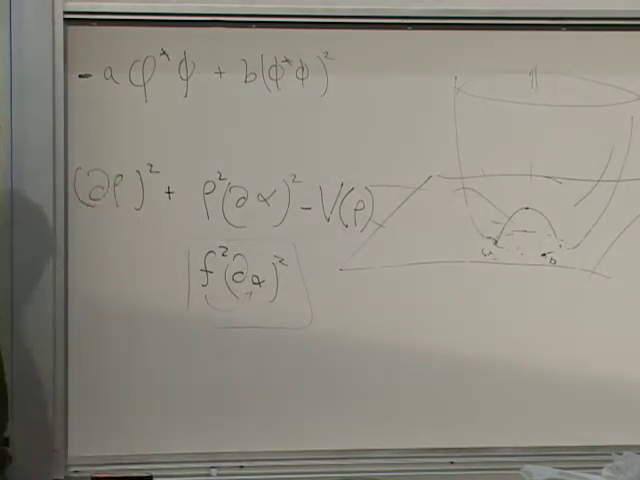
\includegraphics[width=0.88\textwidth]{lecture_07_figure_03.png}
\caption{極座標場的拉格朗日量、框出的低能角向項，以及對稱性破缺勢能。徑向運動會爬升勢能；角向運動則沿著谷底前進。}
\lectureframe{00:56:40}
\end{figure}

對於極低能的激發，場會保持在 \(\rho=f\) 附近。此時
\begin{equation}
  \mathcal L_{\rm angular}
  \simeq f^2(\partial_\mu\alpha)(\partial^\mu\alpha).
\end{equation}
依照因子 \(1/2\) 的選用慣例，定義正則歸一化的角向場為
\begin{equation}
  \beta=\sqrt{2}\,f\alpha,
  \qquad
  \mathcal L_{\rm angular}
  =\frac12(\partial_\mu\beta)(\partial^\mu\beta).
  \label{eq:l07-goldstone-field}
\end{equation}
這裡沒有 \(\beta^2\) 項。這個角向場的量子是無質量的，也就是戈德斯通玻色子。

徑向場的行為則不同。若將 \(\rho\) 從 \(f\) 處處往外移，它會滾回、越過谷底，再繞著谷底振盪。若 \(\rho=f+h\)，將它代入式~\eqref{eq:l07-mexican-hat}展開後可得
\begin{equation}
  V(f+h)=V(f)+\frac12m_h^2h^2+\cdots,
\end{equation}
因此 \(h\) 具有質量。從幾何上看，角向是平坦的，徑向則是彎曲的。

\begin{classroomqa}
\audiencequestion{如果場沿徑向偏離，會直接落回去嗎？接下來會發生什麼？\lecturetimestamp{00:57:10}}
\lecturerresponse{若沒有角向運動，場會朝極小值落下，越過極小值後再作徑向振盪。均勻振盪的空間動量為零，但頻率不為零；這個頻率就是徑向激發的質量。相較之下，均勻的角向位移會落在另一個真空上，沒有回復力。}
\end{classroomqa}

在這個例子中，戈德斯通原理的內容是：自發破缺連續全域對稱性時，真空流形上的每一個獨立平坦方向都會產生一個無質量模式。
\editorialnote{這項說法以相對論場論的通常條件為前提。在非相對論多體系統中，南部--戈德斯通模式的數目和色散關係可能更為微妙；不過，對這個相對論性的\(U(1)\)模型而言，本講關於長波長的結論仍然成立。}

\section{自旋波、弦波與聲波}

這個定理雖然抽象，背後的機制卻很熟悉。在各向同性鐵磁體中，所有自旋一起旋轉並不會改變能量。若取向在樣品中緩慢變化，就會形成自旋波。它的能量代價會隨波數趨近於零，因此它是自旋旋轉對稱性破缺所產生的戈德斯通模式。

長彈性弦則提供另一種圖像。忽略重力，並架設弦的兩端，使整條弦能夠沿垂直方向平移。整條弦均勻地垂直平移不耗能。若平移量沿著弦緩慢改變，就會形成長波長的橫波。原本均勻的對稱操作於是延伸成隨位置緩慢變化的形變。

\begin{figure}[htbp]
\centering
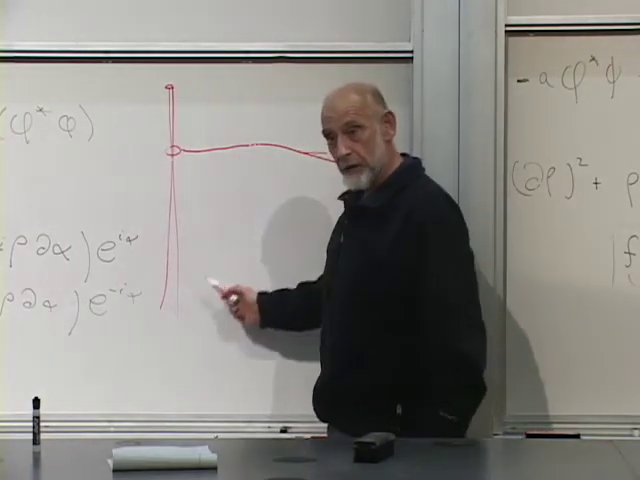
\includegraphics[width=0.68\textwidth]{lecture_07_figure_04.png}
\caption{戈德斯通模式類比中所畫的緩慢變化弦形。物理上的重點是長波長形變的斜率很小，而不是曲線在垂直方向上的位置。}
\lectureframe{01:04:19}
\end{figure}

\begin{classroomqa}
\audiencequestion{弦能否在動量為零時仍帶有振盪能量？\lecturetimestamp{01:04:41}}
\lecturerresponse{必須區分垂直方向的機械動量，以及沿弦傳播的波動動量。駐波可以是 \(+k\) 與 \(-k\) 模式的疊加，因此淨動量為零，但仍然帶有能量。在場論類比中，動量指沿著軸向的波數；垂直位移則代表內部場座標。}
\end{classroomqa}

彈簧玩具可以呈現縱波的情形。將理想化的無限長彈簧玩具沿軸向整體平移，狀態不會改變。若相鄰部分的平移量略有不同，就會形成平緩的壓縮波。在固體或流體中，長波長聲波同樣來自集體位移和密度變化。自旋波、弦的橫波和聲波並不是相同的微觀激發，但它們有一個關鍵共通點：均勻的連續操作不耗能，而緩慢變化的操作則形成軟模式。
\editorialnote{在晶體中，聲學聲子通常被描述為自發破缺連續平移對稱性所產生的南部--戈德斯通模式。講課中以弦和彈簧玩具作為力學類比，說明相同的僅含導數能量結構。}

這些術語很容易混淆，因此課堂上開了個簡短的玩笑：它們是\emph{戈德斯通}玻色子，以 Jeffrey Goldstone 命名，不是規範玻色子。講課中提到 Goldstone 是 Susskind 的朋友，接著便轉向真正不同的主題：規範不變性。

\section{從全域相位對稱性到規範對稱性}

\(U(1)\)相位對稱性在本課程中已經作為與電荷守恆相關的對稱性出現過。帶電粒子的場是複數場，將這樣的場乘上共同相位，不會改變全域理論。為了方便理解，可以把這個電荷想成電荷；不過，它也可能代表其他 \(U(1)\) 量子數。真實的光子是無質量的；我們最終要探討的目標，是像光子一樣的場，例如有質量的 \(Z\)。

新的問題是，
\begin{equation}
  \phi'(x)=e^{i\theta(x)}\phi(x)
  \label{eq:l07-local-u1}
\end{equation}
當 \(\theta\) 在時空中任意變化時，這還能是一種對稱性嗎？函數 \(\theta(x)\) 是變換參數，不是額外的動力學場。我們對它微分，來檢驗這個設想：
\begin{equation}
  \partial_\mu\phi'
  =e^{i\theta}
   \left[\partial_\mu\phi+i(\partial_\mu\theta)\phi\right].
  \label{eq:l07-local-derivative}
\end{equation}
若 \(\theta\) 為常數，就不會出現這個額外項。對共軛場而言，
\begin{equation}
  \partial_\mu\phi^{*\prime}
  =e^{-i\theta}
   \left[\partial_\mu\phi^*-i(\partial_\mu\theta)\phi^*\right].
\end{equation}
兩者相乘後得到
\begin{align}
  \partial_\mu\phi^{*\prime}\partial^\mu\phi'
  ={}&
  \partial_\mu\phi^*\partial^\mu\phi
  i\left(
      \phi\,\partial_\mu\phi^*
      -\phi^*\partial_\mu\phi
    \right)\partial^\mu\theta
  \nonumber\\
  &+\phi^*\phi\,
    \partial_\mu\theta\,\partial^\mu\theta.
  \label{eq:l07-local-failure}
\end{align}
勢能仍保持不變，因為 \(\phi^*\phi\) 不變，但普通的動能項不再保持不變。全域對稱性不會自動成為局域對稱性。

\begin{classroomqa}
\audiencequestion{在墨西哥帽的圖像中，這種不變性失效是否代表環形谷底上有起伏？\lecturetimestamp{01:19:37}}
\lecturerresponse{不是。勢能在角向仍然可以完全平坦。額外的能量代價來自相位在不同時空位置有所差異時產生的梯度。這不是谷底變得凹凸不平，而是普通導數項會感受到空間變化。}
\end{classroomqa}

\subsection{補償用的向量場}

自然界中的 \(W\)、\(Z\) 和膠子交互作用，是由局域規範對稱性組織起來的，不只是由整體變換決定。若要讓局域相位操作成為對稱性，就必須在理論中加入四向量場 \(A_\mu\)。在電磁學中，\(A_0\) 是純量勢，另外三個空間分量則構成向量勢。它們的導數會形成電場和磁場。

採用前後一致的慣例：
\begin{equation}
  \phi'=e^{i\theta}\phi,
  \qquad
  A'_\mu=A_\mu-\partial_\mu\theta,
  \qquad
  D_\mu=\partial_\mu+iA_\mu.
  \label{eq:l07-gauge-convention}
\end{equation}
黑板上檢查抵消時曾改變一個符號；式\eqref{eq:l07-gauge-convention}則將三個符號一併確定。規範耦合和電荷暫時都吸收到 \(A_\mu\) 中。
\editorialnote{若明確寫出電荷 \(q\) 和耦合常數 \(g\)，可以寫成
\(D_\mu=\partial_\mu+igqA_\mu\) 和
\(A'_\mu=A_\mu-(gq)^{-1}\partial_\mu\theta\)。講課中略去這些常數，讓抵消關係更清楚。}

對共軛場而言，
\begin{equation}
  D_\mu\phi^*=\partial_\mu\phi^*-iA_\mu\phi^*.
\end{equation}
現在
\begin{align}
  D'_\mu\phi'
  &=
  \left(\partial_\mu+iA'_\mu\right)e^{i\theta}\phi
  \nonumber\\
  &=
  e^{i\theta}
  \left[
    \partial_\mu\phi+i(\partial_\mu\theta)\phi
    +i(A_\mu-\partial_\mu\theta)\phi
  \right]
  \nonumber\\
  &=e^{i\theta}D_\mu\phi.
  \label{eq:l07-covariant-transform}
\end{align}
\(\theta\) 的多餘導數項會由 \(A_\mu\) 的變換抵消。同樣地，
\begin{equation}
  D'_\mu\phi^{*\prime}=e^{-i\theta}D_\mu\phi^*.
\end{equation}
兩者相乘後保持不變。「\emph{協變}」的意思是，導數的變換方式與場本身相同而簡單。

\section{規範場的動力學}

若引入 \(A_\mu\) 只是為了修正導數，它本身就不會有動力學。規範不變的場強為
\begin{equation}
  F_{\mu\nu}
  =\partial_\mu A_\nu-\partial_\nu A_\mu.
  \label{eq:l07-field-strength}
\end{equation}
它是反對稱的，因此 \(F_{\mu\mu}=0\)。它的時間--空間分量包含電場，空間--空間分量則包含磁場。用熟悉的三維向量表示法來說，電磁場的能量密度正比於 \(\bm E^2+\bm B^2\)，而洛侖茲形式的拉格朗日量正比於 \(\bm E^2-\bm B^2\)；正負號取決於度規慣例。

\begin{classroomqa}
\audiencequestion{電磁場的能量和拉格朗日量分別是什麼？\lecturetimestamp{01:33:20}}
\lecturerresponse{能量由 \(E^2+B^2\) 組成；拉格朗日量則使用 \(E^2-B^2\)。以協變形式表示，後者通常寫成 \(F_{\mu\nu}F^{\mu\nu}\) 的倍數。反對稱張量就是向量勢的四維旋度。}
\end{classroomqa}

場強本身也具有規範不變性：
\begin{align}
  F'_{\mu\nu}
  &=
  \partial_\mu(A_\nu-\partial_\nu\theta)
  -\partial_\nu(A_\mu-\partial_\mu\theta)
  \nonumber\\
  &=
  F_{\mu\nu}
  -\partial_\mu\partial_\nu\theta
  +\partial_\nu\partial_\mu\theta
  =F_{\mu\nu}.
  \label{eq:l07-field-strength-invariant}
\end{align}
最後一個等號成立，是因為普通的混合偏導數可以交換次序。因此，標準的規範不變拉格朗日量可以寫成
\begin{equation}
  \boxed{
  \mathcal L
  =(D_\mu\phi)^*D^\mu\phi
  -V(\phi^*\phi)
  -\frac14F_{\mu\nu}F^{\mu\nu}}
  \label{eq:l07-scalar-qed}
\end{equation}
至於正負號與歸一化慣例，則取決於所採用的度規。

\begin{figure}[htbp]
\centering
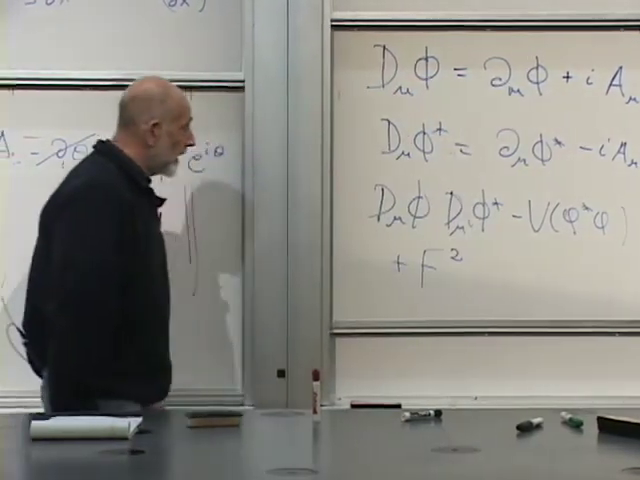
\includegraphics[width=0.84\textwidth]{lecture_07_figure_05.png}
\caption{黑板上的協變導數，以及組合完成的規範不變拉格朗日量。為了清楚呈現變換結構，黑板上的寫法省略了數值因子。}
\lectureframe{01:38:45}
\end{figure}

這個構造將全域 \(U(1)\) 對稱性推廣成局域對稱性，但代價---或者從物理角度來看，這份收穫---是引入一個新的向量場。在阿貝爾例子中，這個場就是電磁勢。

\begin{classroomqa}
\audiencequestion{我們一開始的拉格朗日量使用普通導數。為什麼可以把它們換成協變導數，並把換過之後的結果稱為真正的理論？\lecturetimestamp{01:42:55}}
\lecturerresponse{我們正在構造一個不同且擴充過的理論：帶電物質加上規範場。局域規範不變性決定了兩者的耦合方式。由此得到的量子理論在數學上自成一套一致的結構，也符合自然界對光子和弱作用規範場的組織方式。若不一致地耦合相對論性向量場，可能會引入非物理極化態並破壞機率守恆，因此規範原理並非只是把舊有的自由標量理論重新包裝。}
\end{classroomqa}

\begin{classroomqa}
\audiencequestion{所以，加入新場就是這項修改的根本理由嗎？\lecturetimestamp{01:44:57}}
\lecturerresponse{是的。沒有\(A_\mu\)時，局域轉動後的場，其導數會含有一個未被抵消的\(\partial_\mu\theta\)。加入\(A_\mu\)及其變換律後，這個項就能抵消。用幾何語言來說，\(A_\mu\)是叢上的聯絡；這套更深層的數學確實有其意義，也很有用，但上面的代數已涵蓋此處所需的部分。}
\end{classroomqa}

\section{為什麼裸規範玻色子質量會被禁止}

對一般的玻色場而言，質量以二次項表示。很容易讓人想加上
\begin{equation}
  \Delta\mathcal L_{\rm Proca}
  =\frac12m^2A_\mu A^\mu.
  \label{eq:l07-proca}
\end{equation}
但在\(A_\mu\mapsto A_\mu-\partial_\mu\theta\)之下，
\begin{equation}
  A'_\mu A^{\mu\prime}
  =
  A_\mu A^\mu
  -2A^\mu\partial_\mu\theta
  +\partial_\mu\theta\,\partial^\mu\theta,
\end{equation}
因此，式~\eqref{eq:l07-proca}並非規範不變。我們不能在保留局域對稱性的同時，任意將質量項加進這個規範理論。

\begin{figure}[htbp]
\centering
\includegraphics[width=0.72\textwidth]{lecture_07_figure_07.png}
\caption{所提議的裸向量質量項為\(\tfrac12m^2A_\mu A^\mu\)。此項在\(A_\mu\mapsto A_\mu-\partial_\mu\theta\)之下不再保持不變，這正是希格斯機制所要克服的障礙。}
\lectureframe{01:39:48}
\end{figure}

這就是表面上的僵局。規範不變性說明了光子為何無質量，也保護理論不受非物理自由度的影響；然而，\(W\)和\(Z\)卻有質量。解決之道不能是顯式加入向量質量項，而必須來自規範不變拉格朗日量中原有的場。

\begin{classroomqa}
\audiencequestion{引入規範不變性本身會產生戈德斯通玻色子嗎？\lecturetimestamp{01:45:51}}
\lecturerresponse{不會。向量勢引入之前，連續的\emph{整體}對稱性自發破缺時，就已經產生了戈德斯通玻色子。對稱性一旦成為局域對稱性，相位的變化就可以由\(A_\mu\)補償。在對稱性破缺的規範理論中，角向模式不再是獨立的無質量粒子；它提供了如今有質量的向量場所需的額外極化。下一講將推導這個結果，而不只把它說出來。}
\end{classroomqa}

\begin{classroomqa}
\audiencequestion{這些內容能解釋河流為什麼蜿蜒嗎？\lecturetimestamp{01:47:03}}
\lecturerresponse{目前沒有已知的直接關聯。流體渦旋乃至生物體的形狀，當然都可以用對稱性方法描述；在意想不到的地方發現場論思想，也不值得驚訝。不過，本講並未主張存在描述河流蜿蜒的規範理論。}
\end{classroomqa}

\section{本講到此為止}

我們現在已經具備了開頭所承諾的兩個要素。具有一圈真空態的連續整體對稱性，會有一個平坦的角向方向；這個方向的緩慢變化就是無質量的戈德斯通場。局域對稱性則要求引入規範聯絡與協變導數，並禁止式~\eqref{eq:l07-proca}中的直接向量質量項。

下一步是將式~\eqref{eq:l07-mexican-hat}中的破缺勢，放進式~\eqref{eq:l07-scalar-qed}所描述的規範不變理論中。接著會有兩件事同時發生：獨立的戈德斯通粒子從物理譜中消失，而向量場獲得質量。按照一般的教學說法，規範對稱性自發破缺了；更精確地說，規範冗餘仍然存在，而理論進入希格斯相，其中有一個有質量的向量激發。\editorialnote{局域規範對稱性是描述上的冗餘，不是作用於不同可觀測態之間的一般物理對稱性。本講採用「規範對稱性自發破缺」這個標準簡稱。規範不變的物理陳述則是：希格斯相中的自由度重新組合。}

這就是希格斯現象。我們還沒有推導它。本講完成了必要而更為困難的工作，讓問題變得足夠精確；如此一來，解答出現時便勢所必然。
